%!TEX program = xelatex
\documentclass[11pt, a4paper]{article}

% AA LINGUA E GESTIONE FONT (Specifica per XeLaTeX)
\usepackage{fontspec}
\setmainfont{Latin Modern Roman}
\usepackage[italian]{babel}

% AA LAYOUT DI PAGINA E TIPOGRAFIA (Ottimizzato per Rilegatura)
\usepackage[left=2.4cm, right=1.6cm, top=2cm, bottom=2cm]{geometry}

% AA Spaziatura tra paragrafi controllata (compatta ed evita salti enormi)
\usepackage[skip=3pt plus 1pt minus 1pt]{parskip}
\setlength{\parindent}{0pt}

% AA Microtype per XeLaTeX
\usepackage[protrusion=true]{microtype}
\raggedbottom

% AA GESTIONE DEI COLORI
\usepackage{xcolor}

% AA MATEMATICA E SIMBOLI
\usepackage{amsmath}
\usepackage{mathtools}
\usepackage{silence}
\usepackage[warnings-off={mathtools-overbracket,mathtools-colon}]{unicode-math}
\setmathfont{Latin Modern Math}

% BB OTTIMIZZAZIONE MATRICI LUNGHE PER LA STAMPA
\setlength{\arraycolsep}{10pt}

% AA Spaziature verticali attorno alle formule matematiche
\setlength{\abovedisplayskip}{3pt plus 1pt minus 1pt}
\setlength{\belowdisplayskip}{3pt plus 1pt minus 1pt}
\setlength{\abovedisplayshortskip}{0pt plus 1pt}
\setlength{\belowdisplayshortskip}{2pt plus 1pt minus 1pt}

% AA GRAFICA ED IMMAGINI
\usepackage{graphicx}
\graphicspath{{./E3_6_2_Images/}}

% AA PERSONALIZZAZIONE TITOLI
\usepackage{titlesec}
\titleformat{\section}{\normalfont\Large\bfseries\color{blue!80!black}}{\thesection}{1em}{}
\titleformat{name=\section,numberless}{\normalfont\Large\bfseries\color{blue!80!black}}{}{0pt}{}

\titleformat{\subsection}{\normalfont\large\bfseries}{\thesubsection}{1em}{}
\titleformat{name=\subsection,numberless}{\normalfont\large\bfseries}{}{0pt}{}

\titleformat{\subsubsection}{\normalfont\normalsize\bfseries}{\thesubsubsection}{1em}{}
\titleformat{name=\subsubsection,numberless}{\normalfont\normalsize\bfseries}{}{0pt}{}

\titlespacing*{\section}{0pt}{1.2ex plus 0.4ex minus 0.2ex}{0.6ex plus 0.2ex}
\titlespacing*{\subsection}{0pt}{1ex plus 0.3ex minus 0.2ex}{0.5ex plus 0.2ex}
\titlespacing*{\subsubsection}{0pt}{0.8ex plus 0.2ex minus 0.1ex}{0.4ex plus 0.1ex}

\titleformat{\paragraph}[block]{\normalfont\normalsize\bfseries\color{black!80!black}\raggedright}{}{0pt}{}
\titlespacing*{\paragraph}{0pt}{1.2ex plus 0.3ex minus 0.2ex}{0.4ex}

% AA INTEGRAZIONE CODICE MATLAB
\usepackage{matlab}

% BB Riconfigurazione Automatica Titoli Esportati da MATLAB
\renewcommand{\matlabheading}[1]{\section*{#1}}
\renewcommand{\matlabheadingtwo}[1]{\subsection*{#1}}
\renewcommand{\matlabheadingthree}[1]{\subsubsection*{#1}}

% BB Formule E Matrici Simboliche
\renewenvironment{matlabsymbolicoutput}{%
  \par\vspace{2pt}%
  \begingroup
  \centering
}{%
  \par\vspace{2pt}%
  \endgroup
}

% BB Output Testuale Console
\renewenvironment{matlaboutput}{%
  \par\vspace{1pt}%
  \Verbatim[xleftmargin=10pt, formatcom=\color{black!75}, fontsize=\footnotesize]%
}{%
  \endVerbatim
  \vspace{1pt}%
}

% BB Box Codice (Stile Moderno con Barra Laterale Colorata)
\lstset{
  backgroundcolor={},
  aboveskip=0pt,
  belowskip=0pt,
  basicstyle=\ttfamily\footnotesize,
  xleftmargin=0pt
}

\mdfdefinestyle{matlabcode}{%
  topline=false,
  bottomline=false,
  rightline=false,
  leftline=true,
  linewidth=2.5pt,
  linecolor=blue!75!black,
  backgroundcolor=black!3,
  innertopmargin=4pt,
  innerbottommargin=4pt,
  innerleftmargin=9pt,
  innerrightmargin=6pt,
  skipabove=3pt,
  skipbelow=3pt
}

\allowdisplaybreaks

% AA LINK, METADATI ED ELENCHI
\usepackage{hyperref}
\hypersetup{
    colorlinks=true,
    linkcolor=blue!80!black,
    urlcolor=blue!80!black,
    citecolor=blue!80!black,
    pdftitle={Disaccoppiamento Polso Struttura Portante},
    pdfauthor={Francesco Lo Verde},
}
\usepackage{bookmark}

% BB Spaziatura Elenchi (Arieggiata per la Stampa)
\usepackage{enumitem}
\setlist{itemsep=3.5pt plus 1pt minus 1pt, topsep=4pt plus 1pt minus 1pt, partopsep=0pt, parsep=1pt}


\author{Francesco Lo Verde}
\begin{document}

% \begin{matlabcode}
% clc; clear; close all;
% \end{matlabcode}

\subsection*{CINEMATICA DIRETTA MANIPOLATORE SFERICO}

\begin{par}
    \begin{figure}[!htbp]
        \centering
        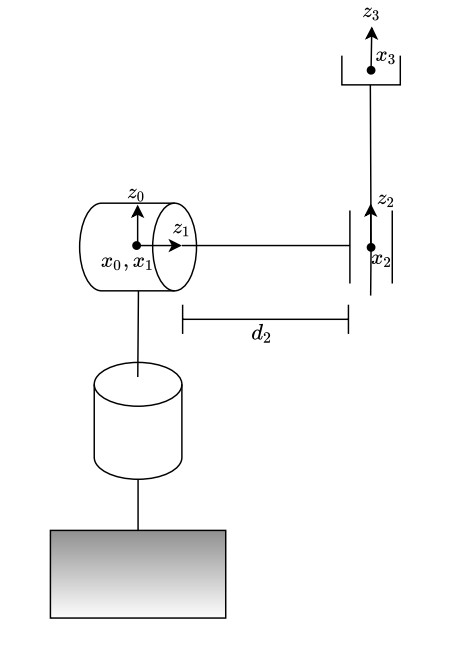
\includegraphics[width=0.5\linewidth]{image_0.jpeg}
    \end{figure}
\end{par}

\begin{matlabcode}
% Definizione Variabili Simboliche
syms q1 q2 q3 d1 d2 d3 alpha1 alpha2 alpha3 a1 a2 a3 real;

DH_table_Strut = [q1, 0, -pi/2, 0;
                  q2, d2, pi/2, 0;
                  0, q3, 0, 0];


% Numero Giunti Manipolatore
n = size(DH_table_Strut, 1);

% Calcolo Matrici Trasformazione Struttura
[T_matrices_Strut, R_matrices_Polso] = Compute_DH_Transformations(DH_table_Strut);
% Visualizzazione Matrici Trasformazione Struttura
j = 0;
for i = 1:n
    fprintf('Matrice Di Trasformazione Omogenea ^{%d}T_(%d):\n', j, j+1);
    disp(T_matrices_Strut(:,:,i));
    j = j+1;
end
\end{matlabcode}
\begin{matlaboutput}
Matrice Di Trasformazione Omogenea ^{0}T_(1):
\end{matlaboutput}
\begin{matlabsymbolicoutput}
\hskip1em $\displaystyle \left(\begin{array}{cccc}
\cos \left(q_1 \right) & 0 & -\sin \left(q_1 \right) & 0\\
\sin \left(q_1 \right) & 0 & \cos \left(q_1 \right) & 0\\
0 & -1 & 0 & 0\\
0 & 0 & 0 & 1
\end{array}\right)$
\end{matlabsymbolicoutput}
\newpage
\begin{matlaboutput}
Matrice Di Trasformazione Omogenea ^{1}T_(2):
\end{matlaboutput}
\begin{matlabsymbolicoutput}
\hskip1em $\displaystyle \left(\begin{array}{cccc}
\cos \left(q_2 \right) & 0 & \sin \left(q_2 \right) & 0\\
\sin \left(q_2 \right) & 0 & -\cos \left(q_2 \right) & 0\\
0 & 1 & 0 & d_2 \\
0 & 0 & 0 & 1
\end{array}\right)$
\end{matlabsymbolicoutput}
\begin{matlaboutput}
Matrice Di Trasformazione Omogenea ^{2}T_(3):
\end{matlaboutput}
\begin{matlabsymbolicoutput}
\hskip1em $\displaystyle \left(\begin{array}{cccc}
1 & 0 & 0 & 0\\
0 & 1 & 0 & 0\\
0 & 0 & 1 & q_3 \\
0 & 0 & 0 & 1
\end{array}\right)$
\end{matlabsymbolicoutput}
\begin{matlabcode}

% Calcolo Matrice Di Trasformazione Totale Dalla Base All'End Effector
T03 = T_matrices_Strut(:,:,1) * T_matrices_Strut(:,:,2) * T_matrices_Strut(:,:,3);
T03 = simplify(T03);

fprintf('Matrice Di Trasformazione Omogenea ^(0)T_(3):\n');

disp(T03);
\end{matlabcode}
\begin{matlaboutput}
Matrice Di Trasformazione Omogenea ^(0)T_(3):
\end{matlaboutput}
\[
    ^{0}\mathbf{T}_{3}(\textbf{q}) \; = \; ^{0}\mathbf{A}_{1}(q_{1}) \; \cdot \; ^{1}\mathbf{A}_{2}(q_{2}) \; \cdot \; ^{2}\mathbf{A}_{3}(q_{3}) =
\]

\[
    =
    \begin{pmatrix}
        c(q_{1})c(q_{2}) & -s(q_{1}) & c(q_{1})s(q_{2}) & c(q_{1})s(q_{2})q_{3} - s(q_{1})d_{2} \\
        s(q_{1})c(q_{2}) & c(q_{1}) & s(q_{1})s(q_{2}) & s(q_{1})s(q_{2})q_{3} + c(q_{1})d_{2}\\
        -s(q_{2}) & 0 & c(q_{2}) & c(q_{2})q_{3}\\
        0 & 0 & 0 & 1
    \end{pmatrix}
\]

\newpage
\subsection*{CINEMATICA DIRETTA POLSO SFERICO}

\begin{par}
    \begin{figure}[htbp]
        \centering
        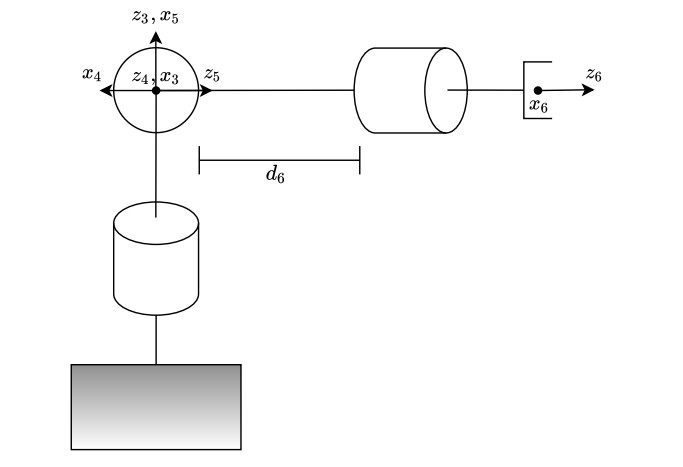
\includegraphics[width=0.75\linewidth]{image_1.jpeg}
    \end{figure}
\end{par}

\begin{matlabcode}
% Definizione Variabili Simboliche
syms q4 q5 q6 d4 d5 d6 alpha4 alpha5 alpha6 a4 a5 a6 real;

% Tabella Parametri Denavit-Hartenberg (DH)
DH_table_Polso = [q4, 0, -pi/2, 0;
                  q5, 0, pi/2, 0;
                  q6, d6, 0, 0];


% Numero Giunti Manipolatore
n = size(DH_table_Polso, 1);

% Calcolo Matrici Trasformazione Polso
[T_matrices_Polso, R_matrices_Polso] = Compute_DH_Transformations(DH_table_Polso);

% Visualizzazione Matrici Trasformazione Polso
j = 3;
for i = 1:n
    fprintf('Matrice Di Trasformazione Omogenea ^(%d)A_(%d):\n', j, j+1);
    disp(T_matrices_Polso(:,:,i));

    j = j+1;
end
\end{matlabcode}
\begin{matlaboutput}
Matrice Di Trasformazione Omogenea ^(3)A_(4):
\end{matlaboutput}
\begin{matlabsymbolicoutput}
\hskip1em $\displaystyle \left(\begin{array}{cccc}
\cos \left(q_4 \right) & 0 & -\sin \left(q_4 \right) & 0\\
\sin \left(q_4 \right) & 0 & \cos \left(q_4 \right) & 0\\
0 & -1 & 0 & 0\\
0 & 0 & 0 & 1
\end{array}\right)$
\end{matlabsymbolicoutput}
\newpage
\begin{matlaboutput}
Matrice Di Trasformazione Omogenea ^(4)A_(5):
\end{matlaboutput}
\begin{matlabsymbolicoutput}
\hskip1em $\displaystyle \left(\begin{array}{cccc}
\cos \left(q_5 \right) & 0 & \sin \left(q_5 \right) & 0\\
\sin \left(q_5 \right) & 0 & -\cos \left(q_5 \right) & 0\\
0 & 1 & 0 & 0\\
0 & 0 & 0 & 1
\end{array}\right)$
\end{matlabsymbolicoutput}
\begin{matlaboutput}
Matrice Di Trasformazione Omogenea ^(5)A_(6):
\end{matlaboutput}
\begin{matlabsymbolicoutput}
\hskip1em $\displaystyle \left(\begin{array}{cccc}
\cos \left(q_6 \right) & -\sin \left(q_6 \right) & 0 & 0\\
\sin \left(q_6 \right) & \cos \left(q_6 \right) & 0 & 0\\
0 & 0 & 1 & d_6 \\
0 & 0 & 0 & 1
\end{array}\right)$
\end{matlabsymbolicoutput}
\begin{matlabcode}

T36 = T_matrices_Polso(:,:,1) * T_matrices_Polso(:,:,2) * T_matrices_Polso(:,:,3);
T36 = simplify(T36);

fprintf('Matrice Di Trasformazione Omogenea ^{3}T_(6):\n');

disp(T36);
\end{matlabcode}
\begin{matlaboutput}
Matrice Di Trasformazione Omogenea ^{3}T_(6):
\end{matlaboutput}
\[
    ^{3}\mathbf{T}_{6}(\textbf{q}) \; = \; ^{3}\mathbf{A}_{4}(q_{4}) \; \cdot \; ^{4}\mathbf{A}_{5}(q_{5}) \; \cdot \; ^{5}\mathbf{A}_{6}(q_{6}) =
\]

\[
    =
        \begin{pmatrix}
            c(q_{4})c(q_{5})c(q_{6}) - s(q_{4})s(q_{6}) & -c(q_{6})s(q_{4}) - c(q_{4})c(q_{5})s(q_{6}) & c(q_{4})s(q_{5}) & c(q_{4})s(q_{5})d_{6} \\
            c(q_{4})s(q_{6}) + c(q_{5})c(q_{6})s(q_{4}) & c(q_{4})c(q_{6}) - c(q_{5})s(q_{4})s(q_{6}) & s(q_{4})s(q_{5}) & s(q_{4})s(q_{5})d_{6} \\
            -c(q_{6})s(q_{5}) & s(q_{5})s(q_{6}) & c(q_{5}) & c(q_{5})d_{6} \\
            0 & 0 & 0 & 1
        \end{pmatrix}
\]

\subsection*{VERIFICA CONDIZIONE DI DISACCOPPIAMENTO}

\begin{par}
$$\exists \;{\mathbf{d}}_0 ,\,{\mathbf{d}}_1 \in {\mathbb{R}}^3 \;\;\mid \;\;^3 {\mathbf{d}}_6 =^3 {\mathbf{R}}_6 {\mathbf{d}}_1 +{\mathbf{d}}_0$$
\end{par}

\begin{matlabcode}
% Estrazione Vettore Posizione
d36 = T36(1:3, 4);
d36 = simplify(d03);
fprintf('Vettore Posizione d_{36}:\n');

disp(d36);
\end{matlabcode}
\begin{matlaboutput}
Vettore Posizione d_{36}:
\end{matlaboutput}

\begin{matlabsymbolicoutput}
\hskip1em $\displaystyle \left(\begin{array}{c}
d_6 \,\cos \left(q_4 \right)\,\sin \left(q_5 \right)\\
d_6 \,\sin \left(q_4 \right)\,\sin \left(q_5 \right)\\
d_6 \,\cos \left(q_5 \right)
\end{array}\right)$
\end{matlabsymbolicoutput}
\newpage
\subsection*{CINEMATICA INVERSA POSIZIONE}

\begin{par}
$$^0 {\mathbf{d}}_6 =^0 {\mathbf{R}}_3 \,^3 {\mathbf{d}}_6 +^0 {\mathbf{d}}_3$$
\end{par}

\begin{matlabcode}
% Estrazione Vettore Posizione
d03 = T03(1:3, 4);
d03 = simplify(d03);
fprintf('Vettore Posizione d_{03}:\n');

disp(d03);
\end{matlabcode}
\begin{matlaboutput}
Vettore Posizione d_{03}:
\end{matlaboutput}
\begin{matlabsymbolicoutput}
\hskip1em $\displaystyle \left(\begin{array}{c}
q_3 \,\cos \left(q_1 \right)\,\sin \left(q_2 \right)-d_2 \,\sin \left(q_1 \right)\\
d_2 \,\cos \left(q_1 \right)+q_3 \,\sin \left(q_1 \right)\,\sin \left(q_2 \right)\\
q_3 \,\cos \left(q_2 \right)
\end{array}\right)$
\end{matlabsymbolicoutput}

\subsection*{CINEMATICA INVERSA ORIENTAMENTO}

\[
    {}^{0}\mathbf{R}_6 = {}^{0}\mathbf{R}_3 \cdot {}^{3}\mathbf{R}_{6}
\]

\begin{matlabcode}
% Matrice Di Rotazione R06
R06 = T06(1:3, 1:3);
R06 = simplify(R06);

% Matrice Di Rotazione R03 Trasposta
R03 = T03(1:3, 1:3);
R03 = simplify(R03);
R03_T = transpose(R03);
disp(R03_T);

% Matrice Di Rotazione R36 Calcolata
R36 = R03_T * R06;
R36 = simplify(R36);
fprintf('Matrice Di Rotazione R36 = (R03)^{T} R06 =:\n');
disp(R36);
\end{matlabcode}
\begin{matlaboutput}
Matrice Di Rotazione R36 = (R03)^{T} R06 =:
\end{matlaboutput}

\resizebox{\linewidth}{!}{%
$
    \begin{pmatrix}
        \cos \left(q_4 \right)\,\cos \left(q_5 \right)\,\cos \left(q_6 \right)-\sin \left(q_4 \right)\,\sin \left(q_6 \right) & -\cos \left(q_6 \right)\,\sin \left(q_4 \right)-\cos \left(q_4 \right)\,\cos \left(q_5 \right)\,\sin \left(q_6 \right) & \cos \left(q_4 \right)\,\sin \left(q_5 \right)\\

        \cos \left(q_4 \right)\,\sin \left(q_6 \right)+\cos \left(q_5 \right)\,\cos \left(q_6 \right)\,\sin \left(q_4 \right) & \cos \left(q_4 \right)\,\cos \left(q_6 \right)-\cos \left(q_5 \right)\,\sin \left(q_4 \right)\,\sin \left(q_6 \right) & \sin \left(q_4 \right)\,\sin \left(q_5 \right)\\

        -\cos \left(q_6 \right)\,\sin \left(q_5 \right) & \sin \left(q_5 \right)\,\sin \left(q_6 \right) & \cos \left(q_5 \right)
    \end{pmatrix}
$}


\matlabheading{Caso Singolare $\sin (q_5 )=0$}

\matlabheadingtwo{Caso Singolare $q_5 =0$}

\begin{matlabcode}
% Sostituzione q5 = 0
R36_Zero = subs(R36, q5, 0);
R36_Zero = simplify(R36_Zero);

fprintf('Matrice Di Rotazione R36 Calcolata Con q5 = 0:\n');

disp(R36_Zero);
\end{matlabcode}
\begin{matlaboutput}
Matrice Di Rotazione R36 Calcolata Con q5 = 0:
\end{matlaboutput}

\begin{matlabsymbolicoutput}
\hskip1em $\displaystyle \left(\begin{array}{ccc}
\cos \left(q_4 +q_6 \right) & -\sin \left(q_4 +q_6 \right) & 0\\
\sin \left(q_4 +q_6 \right) & \cos \left(q_4 +q_6 \right) & 0\\
0 & 0 & 1
\end{array}\right)$
\end{matlabsymbolicoutput}
\newpage

\matlabheadingtwo{Caso Singolare $q_5 =\pi$}

\begin{matlabcode}
% Sostituzione q5 = Pi
R36_Pi = subs(R36, q5, pi);
R36_Pi = simplify(R36_Pi);

fprintf('Matrice Di Rotazione R36 Calcolata Con q5 = Pi:\n');

disp(R36_Pi);
\end{matlabcode}
\begin{matlaboutput}
Matrice Di Rotazione R36 Calcolata Con q5 = Pi:
\end{matlaboutput}
\begin{matlabsymbolicoutput}
\hskip1em $\displaystyle \left(\begin{array}{ccc}
-\cos \left(q_4 -q_6 \right) & -\sin \left(q_4 -q_6 \right) & 0\\
-\sin \left(q_4 -q_6 \right) & \cos \left(q_4 -q_6 \right) & 0\\
0 & 0 & -1
\end{array}\right)$
\end{matlabsymbolicoutput}

\end{document}
